%!TEX ROOT = thesis.tex
\chapter {Implementation and Simulation}
\section{Introduction}
In this chapter, the details of implementation process of the project are explained. The process of building the network, the process of data preparation and preprocessing, as well as the training, testing, and validation process are discussed in details. The simulation, a web application, for the project results are demonstrated in this chapter as well.

\section{Implementation}
The implementation process involves the network models construction, data preparation and preprocessing for the training, validation and testing process of the networks. During the implementation process, networks are constructed using two different activation functions, and applied different number of neurons in hidden layer. For the fusion of the models, minimum, maximum and mean function are used to applied in each networks, the function which get the minimum RMSE results is used as the fusion for the models. 

\subsection{Neural Networks Construction}
The ensemble ANNs models are built using R package libraries such as  RSNNS, neural, nnet, neuralnet, caret, rnn, and NeuralNetTools. The two models are constructed to analyze the optimal model for the forecasting.

The homogeneous model is built only using MLPs networks topology with different initial learning weight being applied in each MLPs. The model is also applied two different activation functions which are sigmoid logistic and hyperbolic tangent. The homogeneous model is constructed using MLP function from neuralnet R package library.

The heterogeneous model is constructed using MLPs, RNN, RBF networks topology with different initial learning weight being applied. The model is also applied two different activation functions same like homogeneous model construction. The heterogeneous model is constructed using MLP, RNN, RBF functions from neuralnet, rnn, and neural R package libraries.

After the extensive literature review, one hidden layer is used for both homogeneous and heterogeneous models constructions. For both model, the inputs parameters are based on the predictor order assigned. The initial number of neurons in hidden layer is calculated using the methods which is suggested by \citeA{lawrence:1993}. The number of neurons are limited until twenty for the time being. Two different activation functions and learning rate of 0.1 until 1.0 is used to applied for the both networks models.

For the single ANN models, the predictor order, the number of neurons, activation function, and learning rate are selected based on the optimal homogeneous and heterogeneous models results. The single ANN models is constructed in order to compare  with the performance of ensemble models which are homogeneous and heterogeneous models.

\subsection{Data Preparation and Preprocessing}
Since the approach is purely based on the data-driven approach, the data are prepared and processed based on predictor order which starting from 3 until 10 to give as input parameters for the networks. For example, if the prediction order is three, then the data set will be processed as three days data as inputs data, the fourth-day data as output data. Due to the time and resource limitation, the predictor order  are limited to experiment only 3 until 10. 

After data is being collected into datasets, datasets are normalized between 0 and 1 for the faster performance in training process. Based on the predictor order, the normalized data are being processed using data\_processing function into three different datasets, training datasets, testing datasets, and validation datasets. These three datasets are used to process while training, testing, and validation process of the network models.

To train the networks models, three different data splitting ratio is applied. These three datasets are processed with three ratio using data\_spliting function. In the first separation, it is assigned to 60\%, 20\%, and 20\% for training, testing, and validation respectively. As for the second separation, 70\%, 15\%, and 15\% is used for  training, testing, and validation respectively. For the final ratio, 80\%, 10\%, and 10\% of the dataset is used for  training, testing, and validation respectively.

\subsection{Training, Testing, and Validation Process}

The two models are trained to get specific optimal model for each currency with different ratio. After the models are being trained, the testing datasets are used to test the models. The results from testing process are measured using RSME and MAE for the error and accuracy performance of the models. The optimal models are validated using validation datasets.

The two functions, HOMO and HETERO, is programmed for the ensemble models. Training process used  HOMO function and  HETERO function for each currency. For the both functions, predictor order, learning function, train dataset, validate dataset, non-normalized actual data, number of neurons, activation function, learning rate are applied as parameters.

For each currency, there are 2720 results are generated in each model. Among these results, the lowest RSME error is selected as the optimal model for that currency for the model. Since there are two models, homogeneous and heterogeneous models, there are two optimal models. Both optimal models are also compared with the single models. These two optimal models are then compared again using same principle to select the best optimal model for the research project.

The testing datasets is used to analyze the accuracy of the optimal models. The validation datasets are applied to the optimal models to validate the result finding. They are also utilize for the project simulation. The details of the functions which are applied to train,test, and validate are available in the appendix.
\pagebreak


\section{Simulation}

For this project, simple web application is built to demonstrated the optimal models using Shiny App library package in R. In the web application, users can enter inputs, the historical data, in order to predict next day exchange rate. The inputs are given to the optimal model to predict the next day future exchange rate. 

\begin{figure}[hbt!]\centering
	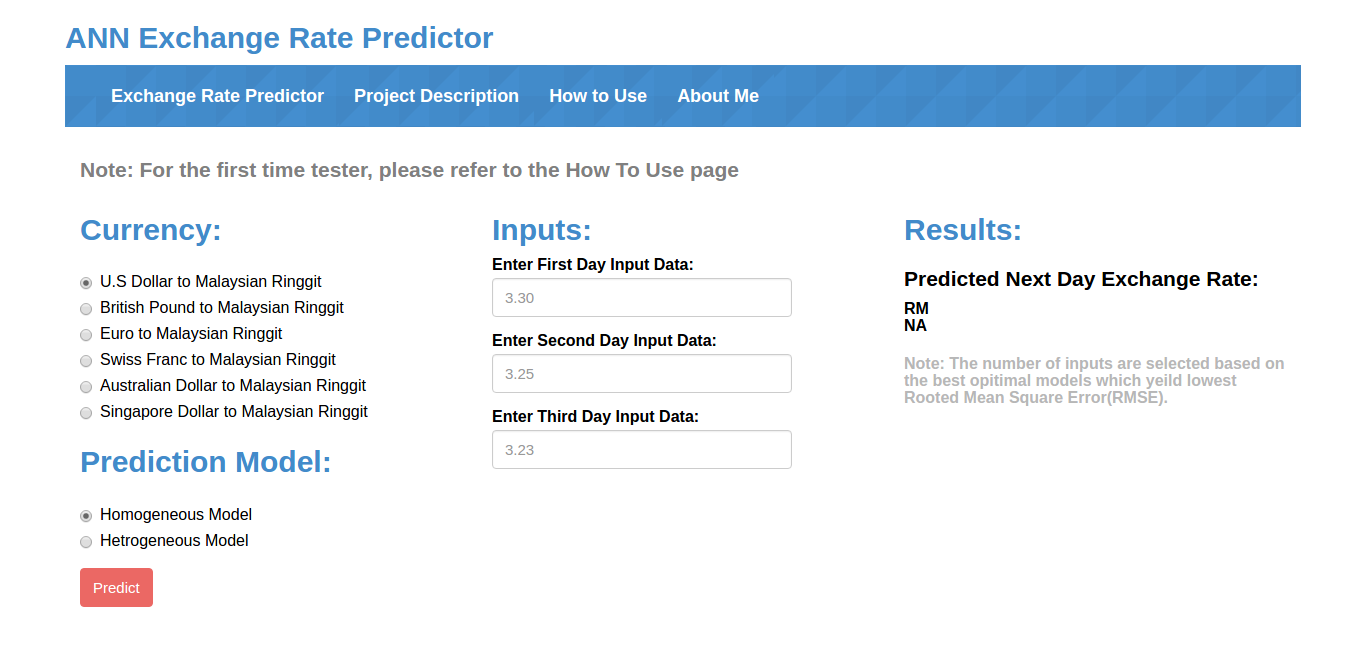
\includegraphics[width=1.1\textwidth]{main}
	\caption{Home page of web application }
\end{figure}

The information on how to test or use the web application is described in the How to Use page of the application. The testing datasets are also provided in the web application for users to test out the application.
\pagebreak

\begin{figure}[hbt!]\centering
	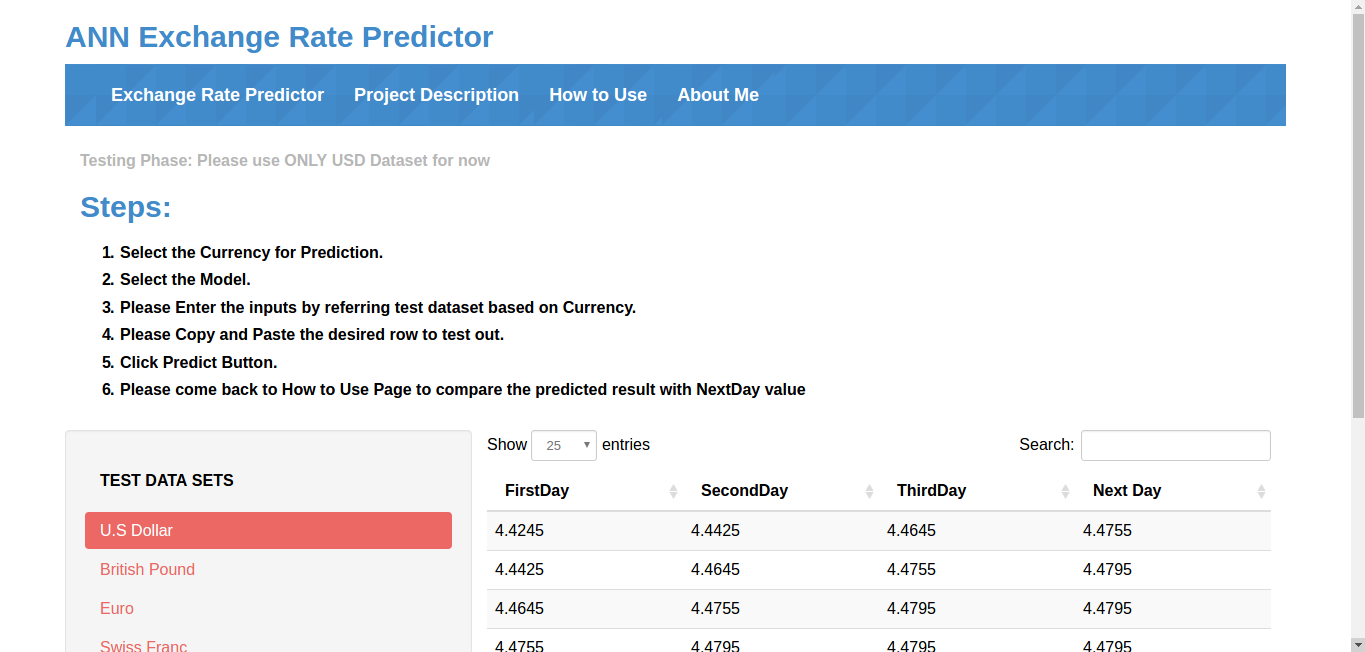
\includegraphics[width=1.1\textwidth]{how_to_use}
	\caption{How to Use page of web application }
\end{figure}

For the USD to RM exchange rates, 4.4425 RM, 4.4645 RM, and 4.4755 RM are selected as first day, second day, and third day inputs data from the table provided by the Test Data Sets. The  next day actual value is  4.4795 RM. The homogeneous model predicted that the value is 4.478467 RM. The error, the difference between these two values is only 0.001033. 

\begin{figure}[hbt!]\centering
	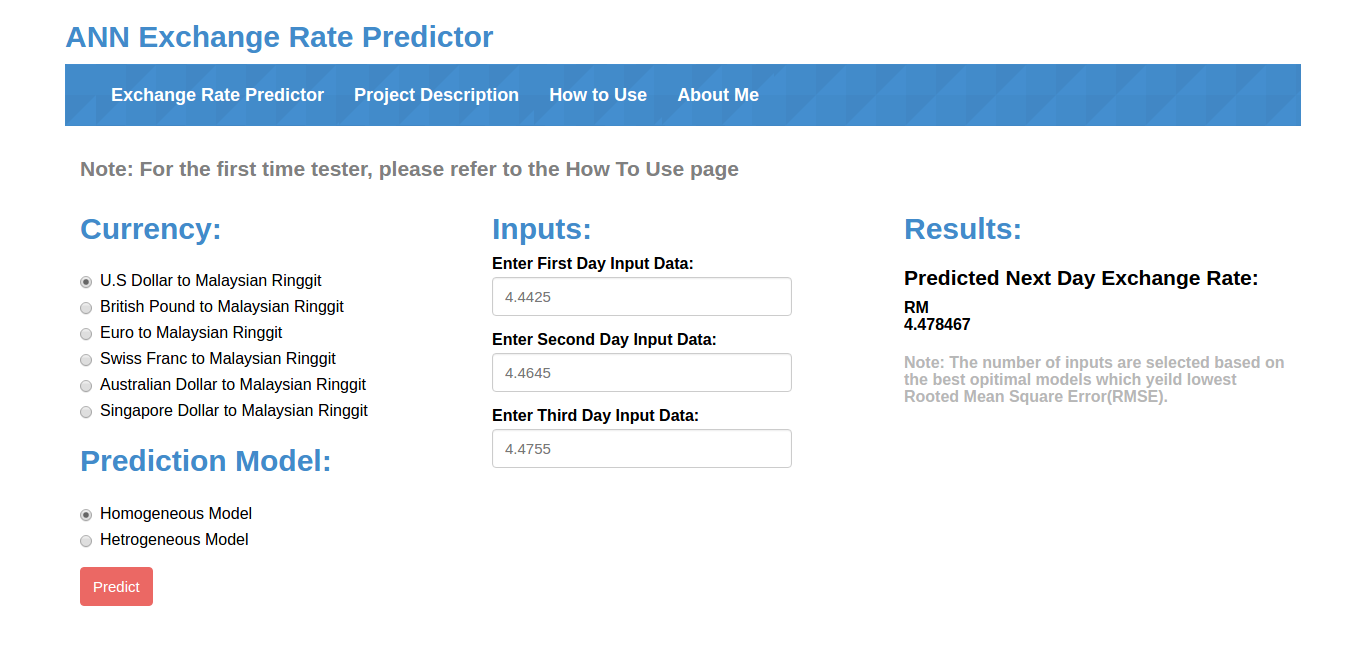
\includegraphics[width=1.1\textwidth]{tested_main}
	\caption{Home page with predicted results based on user inputs}
\end{figure}
\pagebreak

\section{Conclusion}
The implementation is using mainly R programming libraries and tools. Models are being trained  with using different datasets ratio for training, testing, and validation. For each currency, there is one optimal model is selected for each homogeneous and heterogeneous model. The best optimal model is obtained after analyzing different models and the lowest RMSE result is chosen to be the model. A simple web application is also built to demonstrate the optimal models.